\documentclass[a4paper,14pt, unknownkeysallowed]{extreport}

\usepackage{cmap} % Улучшенный поиск русских слов в полученном pdf-файле
\usepackage[T2A]{fontenc} % Поддержка русских букв
\usepackage[utf8]{inputenc} % Кодировка utf8
\usepackage[english,russian]{babel} % Языки: русский, английский
\usepackage{enumitem}


\usepackage{threeparttable}

\usepackage[14pt]{extsizes}

\usepackage{caption}
\captionsetup{labelsep=endash}
\captionsetup[figure]{name={Рисунок}}

% \usepackage{ctable}
% \captionsetup[table]{justification=raggedleft,singlelinecheck=off}

\usepackage{amsmath}

\usepackage{geometry}
\geometry{left=30mm}
\geometry{right=10mm}
\geometry{top=20mm}
\geometry{bottom=20mm}

\usepackage{titlesec}
\titleformat{\section}
	{\normalsize\bfseries}
	{\thesection}
	{1em}{}
\titlespacing*{\chapter}{0pt}{-30pt}{8pt}
\titlespacing*{\section}{\parindent}{*4}{*4}
\titlespacing*{\subsection}{\parindent}{*4}{*4}

\usepackage{setspace}
\onehalfspacing % Полуторный интервал

\frenchspacing
\usepackage{indentfirst} % Красная строка

\usepackage{titlesec}
\titleformat{\chapter}{\LARGE\bfseries}{\thechapter}{20pt}{\LARGE\bfseries}
\titleformat{\section}{\Large\bfseries}{\thesection}{20pt}{\Large\bfseries}

\usepackage{multirow}
\usepackage{listings}
\usepackage{xcolor}

% Для листинга кода:
\lstset{%
	language=Lisp,   					% выбор языка для подсветки	
	basicstyle=\small\sffamily,			% размер и начертание шрифта для подсветки кода
	numbers=left,						% где поставить нумерацию строк (слева\справа)
	numberstyle=\tiny,		     		% размер шрифта для номеров строк
	stepnumber=1,						% размер шага между двумя номерами строк
	numbersep=5pt,						% как далеко отстоят номера строк от подсвечиваемого кода
	frame=single,						% рисовать рамку вокруг кода
	tabsize=4,							% размер табуляции по умолчанию равен 4 пробелам
	captionpos=t,						% позиция заголовка вверху [t] или внизу [b]
	breaklines=true,					
	breakatwhitespace=true,				% переносить строки только если есть пробел
	backgroundcolor=\color{white},
	basicstyle=\footnotesize\ttfamily,
	keywordstyle=\color{blue},
	stringstyle=\color{red},
	commentstyle=\color{gray},
	showspaces=false,
    showstringspaces=false
}


\usepackage{pgfplots}
\usetikzlibrary{datavisualization}
\usetikzlibrary{datavisualization.formats.functions}


\lstset{
	literate=
	{а}{{\selectfont\char224}}1
	{б}{{\selectfont\char225}}1
	{в}{{\selectfont\char226}}1
	{г}{{\selectfont\char227}}1
	{д}{{\selectfont\char228}}1
	{е}{{\selectfont\char229}}1
	{ж}{{\selectfont\char230}}1
	{з}{{\selectfont\char231}}1
	{и}{{\selectfont\char232}}1
	{й}{{\selectfont\char233}}1
	{к}{{\selectfont\char234}}1
	{л}{{\selectfont\char235}}1
	{м}{{\selectfont\char236}}1
	{н}{{\selectfont\char237}}1
	{о}{{\selectfont\char238}}1
	{п}{{\selectfont\char239}}1
	{р}{{\selectfont\char240}}1
	{с}{{\selectfont\char241}}1
	{т}{{\selectfont\char242}}1
	{у}{{\selectfont\char243}}1
	{ф}{{\selectfont\char244}}1
	{х}{{\selectfont\char245}}1
	{ц}{{\selectfont\char246}}1
	{ч}{{\selectfont\char247}}1
	{ш}{{\selectfont\char248}}1
	{щ}{{\selectfont\char249}}1
	{ъ}{{\selectfont\char250}}1
	{ы}{{\selectfont\char251}}1
	{ь}{{\selectfont\char252}}1
	{э}{{\selectfont\char253}}1
	{ю}{{\selectfont\char254}}1
	{я}{{\selectfont\char255}}1
	{А}{{\selectfont\char192}}1
	{Б}{{\selectfont\char193}}1
	{В}{{\selectfont\char194}}1
	{Г}{{\selectfont\char195}}1
	{Д}{{\selectfont\char196}}1
	{Е}{{\selectfont\char197}}1
	{Ж}{{\selectfont\char198}}1
	{З}{{\selectfont\char199}}1
	{И}{{\selectfont\char200}}1
	{Й}{{\selectfont\char201}}1
	{К}{{\selectfont\char202}}1
	{Л}{{\selectfont\char203}}1
	{М}{{\selectfont\char204}}1
	{Н}{{\selectfont\char205}}1
	{О}{{\selectfont\char206}}1
	{П}{{\selectfont\char207}}1
	{Р}{{\selectfont\char208}}1
	{С}{{\selectfont\char209}}1
	{Т}{{\selectfont\char210}}1
	{У}{{\selectfont\char211}}1
	{Ф}{{\selectfont\char212}}1
	{Х}{{\selectfont\char213}}1
	{Ц}{{\selectfont\char214}}1
	{Ч}{{\selectfont\char215}}1
	{Ш}{{\selectfont\char216}}1
	{Щ}{{\selectfont\char217}}1
	{Ъ}{{\selectfont\char218}}1
	{Ы}{{\selectfont\char219}}1
	{Ь}{{\selectfont\char220}}1
	{Э}{{\selectfont\char221}}1
	{Ю}{{\selectfont\char222}}1
	{Я}{{\selectfont\char223}}1
}

\usepackage{graphicx}
\newcommand{\img}[3] {
	\begin{figure}[h!]
		\center{\includegraphics[height=#1]{img/#2}}
		\caption{#3}
		\label{img:#2}
	\end{figure}
}


\usepackage[justification=centering]{caption} % Настройка подписей float объектов

\usepackage[unicode,pdftex]{hyperref} % Ссылки в pdf
\hypersetup{hidelinks}

\usepackage{csvsimple}

\newcommand{\code}[1]{\texttt{#1}}

\usepackage{longtable}

\usepackage{array}
\usepackage{booktabs}
\usepackage{floatrow}

\floatsetup[longtable]{LTcapwidth=table}

% \def\UrlBreaks{\do\/\do-\do\_}

\makeatletter
\renewcommand*\l@chapter[2]{%
  \ifnum \c@tocdepth >\m@ne
    \addpenalty{-\@highpenalty}%
    \vskip 1.0em \@plus\p@
    \setlength\@tempdima{1.5em}%
    \begingroup
      \parindent \z@ \rightskip \@pnumwidth
      \parfillskip -\@pnumwidth
      \leavevmode \bfseries
      \advance\leftskip\@tempdima
      \hskip -\leftskip
      #1\nobreak\normalfont\leaders\hbox{$\m@th
        \mkern \@dotsep mu\hbox{.}\mkern \@dotsep
        mu$}\hfill\nobreak\hb@xt@\@pnumwidth{\hss #2}\par
      \penalty\@highpenalty
    \endgroup
  \fi}
\makeatother

\begin{document}



\begin{titlepage}
	\newgeometry{pdftex, left=2cm, right=2cm, top=2.5cm, bottom=2.5cm}
	\fontsize{12pt}{12pt}\selectfont
	\noindent \begin{minipage}{0.15\textwidth}
		
\includegraphics[width=\linewidth]{img/b_logo.jpg}
	\end{minipage}
	\noindent\begin{minipage}{0.9\textwidth}\centering
		\textbf{Министерство науки и высшего образования Российской Федерации}\\
		\textbf{Федеральное государственное бюджетное образовательное учреждение высшего образования}\\
		\textbf{«Московский государственный технический университет имени Н. Э.~Баумана}\\
		\textbf{(национальный исследовательский университет)»}\\
		\textbf{(МГТУ им. Н. Э.~Баумана)}
	\end{minipage}
	
	\noindent\rule{18cm}{3pt}
	\newline\newline
	\noindent ФАКУЛЬТЕТ $\underline{\text{«Информатика и системы управления»~~~~~~~~~~~~~~~~~~~~~~~~~~~~~~~~~~~~~~~~~~~~~~~~~~~~~~~}}$ \newline\newline
	\noindent КАФЕДРА $\underline{\text{«Программное обеспечение ЭВМ и информационные технологии»~~~~~~~~~~~~~~~~~~~~~~~}}$\newline\newline\newline\newline\newline\newline\newline
	
	
	\begin{center}
		\noindent\begin{minipage}{1.3\textwidth}\centering
		\Large\textbf{   ~~~ Лабораторная работа №4}\newline
		\textbf{по курсу "Функциональное}\newline
		\textbf{и логическое программирование"}\newline\newline\newline
		\end{minipage}
	\end{center}
	
	\noindent\textbf{Тема} 			$\underline{\text{Использование управляющих структур, работа со списками}}$\newline\newline
	\noindent\textbf{Студент} 		$\underline{\text{Ковалец К. Э.}}$\newline\newline
	\noindent\textbf{Группа} 		$\underline{\text{ИУ7-63Б}}$\newline\newline
	\noindent\textbf{Преподаватели} $\underline{\text{Толпинская Н. Б., Строганов Ю. В.}}$\newline
	
	\begin{center}
		\vfill
		Москва~---~\the\year
		~г.
	\end{center}
	\restoregeometry
\end{titlepage}



\setcounter{page}{2}
\chapter{Практические задания}

\section{Задание 1}

Чем принципиально отличаются функции \texttt{cons, list, append}?

Пусть \texttt{(setf lst1 '(a b)) (setf lst2 '(c d))}.
Каковы результаты вычисления следующих выражений?

\begin{center}
\captionsetup{justification=raggedright,singlelinecheck=off}
\begin{lstlisting}[label=lst:parallel_processing,caption=Решение задания 1]
(cons lst1 lst2)   ;; ((A B) C D)
(list lst1 lst2)   ;; ((A B) (C D))
(append lst1 lst2) ;; (A B C D)
\end{lstlisting}
\end{center}

\section{Задание 2}

Каковы результаты вычисления следующих выражений, и почему?

\begin{center}
\captionsetup{justification=raggedright,singlelinecheck=off}
\begin{lstlisting}[label=lst:parallel_processing,caption=Решение задания 2]
(reverse ())         ;; NIL
(last ())            ;; NIL
(reverse '(a))       ;; (A)
(last '(a))          ;; (A)
(reverse '((a b c))) ;; ((A B C))
(last '((a b c)))    ;; ((A B C))
\end{lstlisting}
\end{center}

\clearpage

\section{Задание 3}

Написать, по крайней мере, два варианта функции, которая возвращает последний элемент своего списка-аргумента.

\begin{center}
\captionsetup{justification=raggedright,singlelinecheck=off}
\begin{lstlisting}[label=lst:parallel_processing,caption=Решение задания 3]
(defun last-elem (lst)
    (car (reverse lst)))

;; (LAST-ELEM '(1 2 3)) -> 3

(defun last-elem-2 (lst)
    (if (eq (cdr lst) nil) 
        (car lst) 
    	(last-elem-2 (cdr lst))))

;; (LAST-ELEM-2 '(1 2 3)) -> 3

(defun last-elem-3 (lst)
    (car (last lst)))

;; (LAST-ELEM-3 '(1 2 3)) -> 3
\end{lstlisting}
\end{center}

\section{Задание 4}

Написать, по крайней мере, два варианта функции, которая возвращает свой список-аргумент без последнего элемента.

\begin{center}
\captionsetup{justification=raggedright,singlelinecheck=off}
\begin{lstlisting}[label=lst:parallel_processing,caption=Решение задания 4]
(defun without-last-elem (lst)
    (reverse (cdr (reverse lst))))

;; (WITHOUT-LAST-ELEM '(1 2 3)) -> (1 2)

(defun without-last-elem-2 (lst)
    (if (cdr lst)
        (cons (car lst) (without-last-elem-2 (cdr lst)))
        ()))

;; (WITHOUT-LAST-ELEM-2 '(1 2 3)) -> (1 2)
\end{lstlisting}
\end{center}

\section{Задание 5}

Написать простой вариант игры в кости, в котором бросаются две правильные кости. Если сумма выпавших очков равна 7 или 11 -- выигрыш, если выпало (1,1) или (6,6) -- игрок получает право снова бросить кости, во всех остальных случаях ход переходит ко второму игроку, но запоминается сумма выпавших очков. Если второй игрок не выигрывает абсолютно, то выигрывает тот игрок, у которого больше очков. Результат игры и значения выпавших костей выводить на экран с помощью функции \texttt{print}.

\begin{center}
\captionsetup{justification=raggedright,singlelinecheck=off}
\begin{lstlisting}[label=lst:parallel_processing,caption=Решение задания 5]
(defvar name-first  'first_player)
(defvar name-second 'second_player)
(defvar dice-first)
(defvar dice-second)
(defvar tmp-dice)

(defun roll-one-dice ()
	(+ (random 6) 1))

(defun roll-two-dice ()
	(list (roll-one-dice) (roll-one-dice)))

(defun sum (dice) 
	(+ (car dice) (cadr dice)))

(defun print-res (name dice) 
	(print `(Win ,name)))

(defun is-win (dice) 
	(cond ((= (sum dice) 7 )) 
			((= (sum dice) 11))
	)
)

(defun repeat-roll (dice)
	(cond ((= (car dice) (cadr dice) 6))
			((= (car dice) (cadr dice) 1))
	) 
)

(defun players-move (name)
	(setf tmp-dice (roll-two-dice)
	)
	(print `(,name ,tmp-dice sum = ,(sum tmp-dice))
	)
	(cond 
		((is-win tmp-dice) 
			(list tmp-dice 1))
		((repeat-roll tmp-dice) 
			(players-move name))
		(T (list tmp-dice 0))
	)	
)

(defun continue-game (dice-first)
	(setf dice-second (players-move name-second)
	)
	(cond 
		((= (cadr dice-second) 1) 
			(print-res name-second dice-second))
		((> (sum (car dice-first)) (sum (car dice-second))) 
			(print-res name-first dice-first))
		((< (sum (car dice-first)) (sum (car dice-second))) 
			(print-res name-second dice-second))
		(T (print '(Draw)))
	)
)

(defun play ()
	(setf dice-first  (players-move name-first)
	)
	(cond 
		((= (cadr dice-first) 1) 
			(print-res name-first dice-first))
		(T (continue-game dice-first))
	)
	(terpri) (terpri)
)

;; (FIRST_PLAYER (1 3) SUM = 4) 
;; (SECOND_PLAYER (1 1) SUM = 2) 
;; (SECOND_PLAYER (3 3) SUM = 6) 
;; (WIN SECOND_PLAYER) 

;; (FIRST_PLAYER (1 6) SUM = 7) 
;; (WIN FIRST_PLAYER) 

;; (FIRST_PLAYER (4 6) SUM = 10) 
;; (SECOND_PLAYER (6 4) SUM = 10) 
;; (DRAW) 
\end{lstlisting}
\end{center}


\chapter{Ответы на теоретические вопросы к лабораторной работе}

\section{Синтаксическая форма и хранение программы в памяти}

В Lisp формы представления программы и обрабатываемых ею данных одинаковы и представляются в виде S-выражений. Программы могут обрабатывать и преобразовывать другие программы и сами себя. В процессе трансляции можно введенное и сформированное в результате вычислений выражение данных интерпретировать в качестве программы и непосредственно выполнить. 

Так как программа представляет собой S-выражение, в памяти она представлена либо как атом, либо как точечная пара.

\section{Трактовка элементов списка}

Первый аргумент списка трактуется как имя функции, остальные -- как аргументы этой функции.

\section{Порядок реализации программы}

Программа в языке Lisp представляется S-выражением, которое передается интерпретатору -- функции eval, которая выводит последний, полученный после обработки S-выражения результат. 

Работа функции eval представлена на рисунке \ref{fig:diagram}.

\clearpage
\begin{figure}[h]
	\centering
	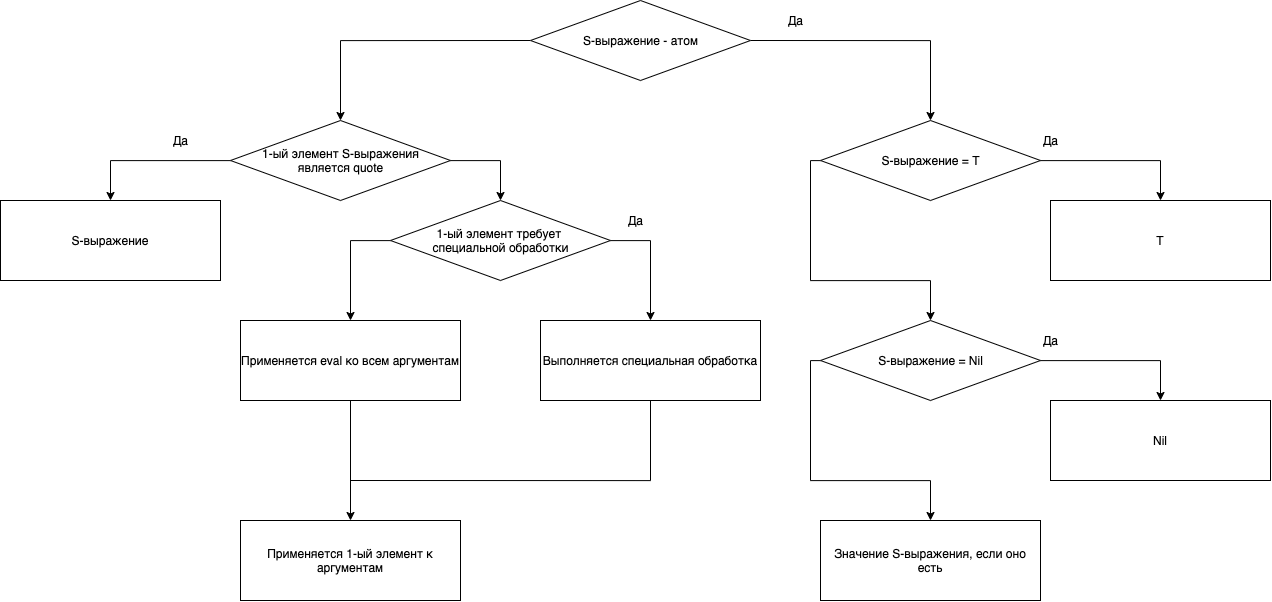
\includegraphics[scale=0.35]{img/diagram.png}
	\caption{Схема работы функции eval}
	\label{fig:diagram}
\end{figure} 

\section{Способы определения функции}

\textbf{Функцией} называется правило, по которому каждому значению одного или нескольких аргументов ставится в соответствие конкретное значение результата.

\begin{itemize}
	\item В Lisp можно определить функцию без имени с помощью \textbf{$\lambda$-выражений}. 
	Lambda-определение безымянной функции:
	
	\begin{center}
	\texttt{(lambda <lambda-список> <форма>)}
	\end{center}

	Lambda-вызов функции:

	\begin{center}
	\texttt{(<lambda-выражение> <формальные параметры>)}
	\end{center}

	\item Также в Lisp можно определить функцию с именем с помощью \textbf{defun}. В таких функциях defun связывает символьный атом с Lambda-определением:
	
	\begin{center}
	\texttt{(defun f <lambda-выражение>)}
	\end{center}

	Упрощенное определение:

	\begin{center}
	\texttt{(defun f(arg1, ..., argN) <формы>)}
	\end{center}

\end{itemize}

\end{document}
